
\tikzset{every picture/.style={line width=0.75pt}} %set default line width to 0.75pt        

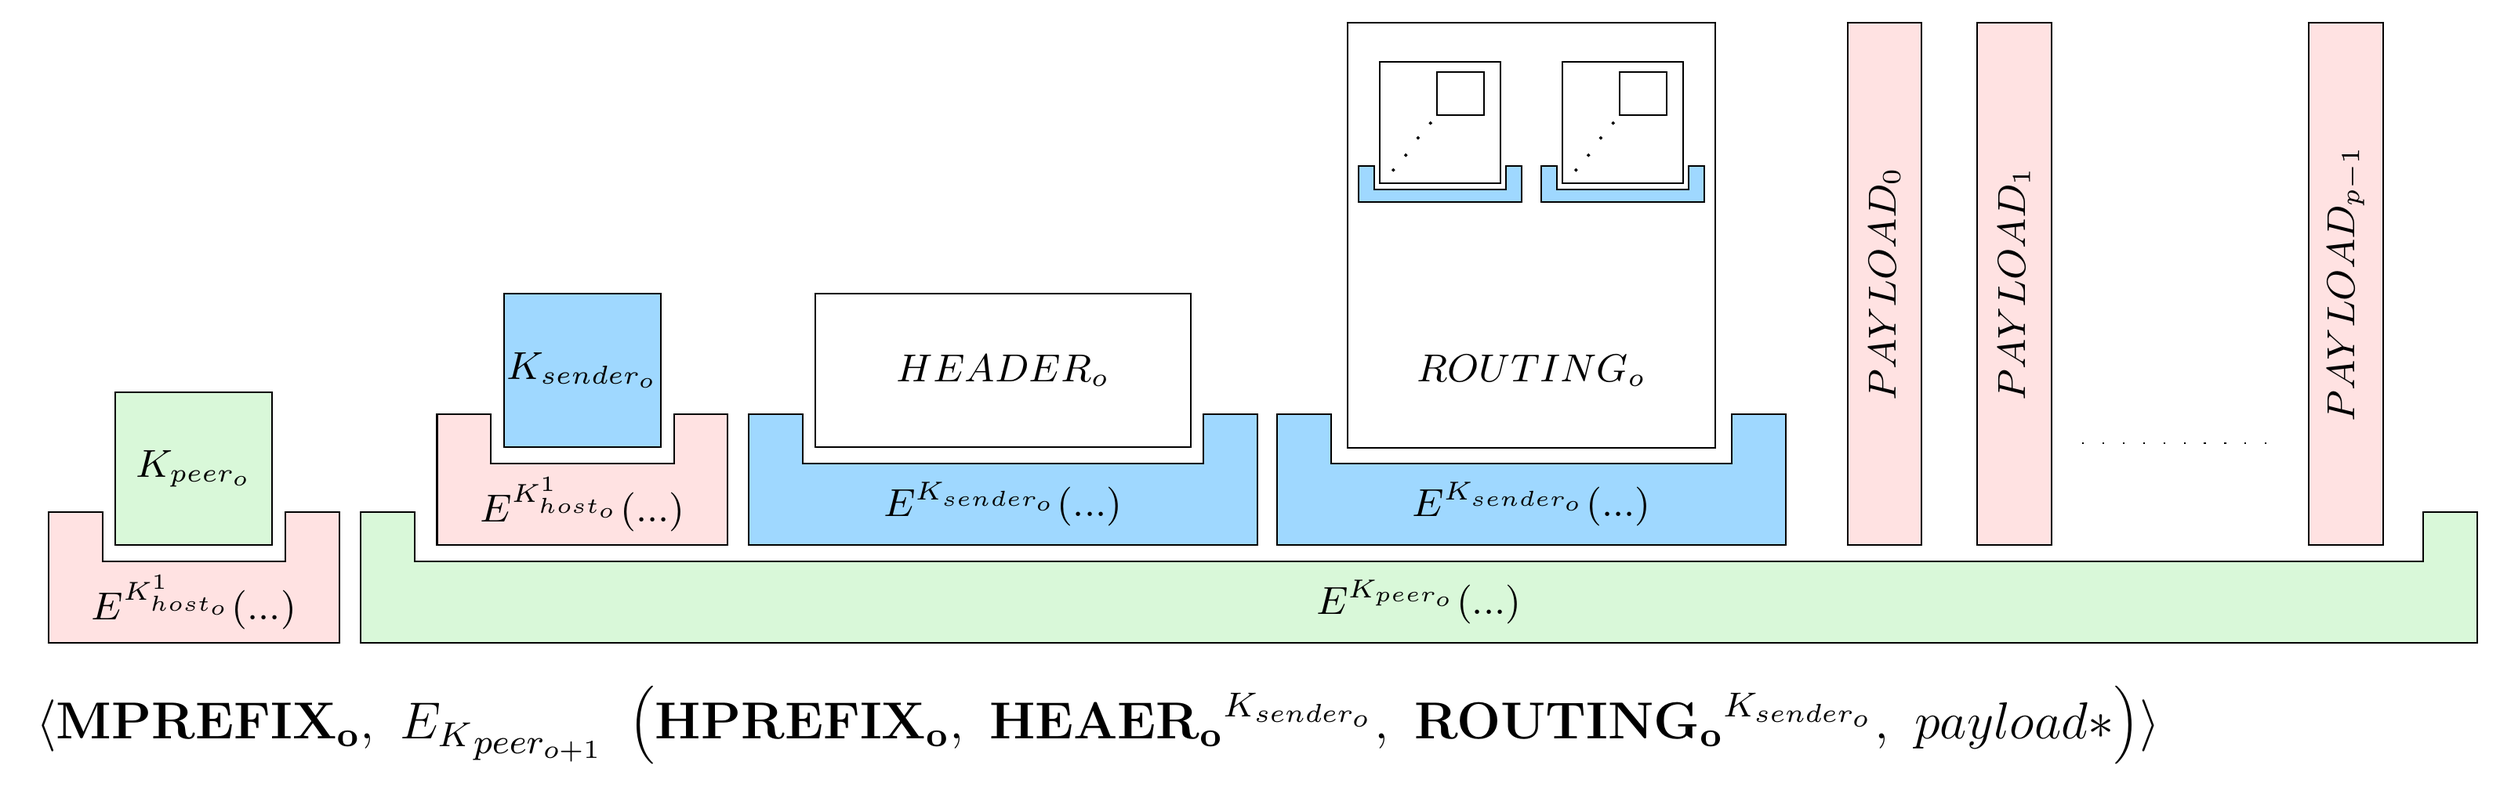
\begin{tikzpicture}[x=0.75pt,y=0.75pt,yscale=-1,xscale=1]
%uncomment if require: \path (0,995); %set diagram left start at 0, and has height of 995

%Shape: Path Data [id:dp2167846330287353] 
\draw  [fill={rgb, 255:red, 255; green, 226; blue, 226 }  ,fill opacity=1 ] (213.69,453.61) -- (213.69,534.21) -- (35,534.21) -- (35,453.61) -- (68.08,453.61) -- (68.08,484.03) -- (180.61,484.03) -- (180.61,453.61) -- (213.69,453.61) -- cycle ;
%Shape: Path Data [id:dp5088749110060282] 
\draw  [fill={rgb, 255:red, 255; green, 226; blue, 226 }  ,fill opacity=1 ] (452.45,393.54) -- (452.45,474.14) -- (273.76,474.14) -- (273.76,393.54) -- (306.84,393.54) -- (306.84,423.96) -- (419.38,423.96) -- (419.38,393.54) -- (452.45,393.54) -- cycle ;
%Shape: Path Data [id:dp2662475941272804] 
\draw  [fill={rgb, 255:red, 159; green, 216; blue, 255 }  ,fill opacity=1 ] (777.9,393.54) -- (777.9,474.14) -- (465.38,474.14) -- (465.38,393.54) -- (498.46,393.54) -- (498.46,423.96) -- (744.82,423.96) -- (744.82,393.54) -- (777.9,393.54) -- cycle ;
%Shape: Path Data [id:dp4996370890622781] 
\draw  [fill={rgb, 255:red, 159; green, 216; blue, 255 }  ,fill opacity=1 ] (1102.58,393.54) -- (1102.58,474.14) -- (790.06,474.14) -- (790.06,393.54) -- (823.14,393.54) -- (823.14,423.96) -- (1069.51,423.96) -- (1069.51,393.54) -- (1102.58,393.54) -- cycle ;
%Shape: Path Data [id:dp6811872237881966] 
\draw  [fill={rgb, 255:red, 217; green, 248; blue, 217 }  ,fill opacity=1 ] (1527.64,453.61) -- (1527.64,534.21) -- (226.62,534.21) -- (226.62,453.61) -- (259.97,453.61) -- (259.97,484.03) -- (1494.56,484.03) -- (1494.56,453.61) -- (1527.64,453.61) -- cycle ;
%Shape: Rectangle [id:dp9628618364963484] 
\draw  [fill={rgb, 255:red, 255; green, 226; blue, 226 }  ,fill opacity=1 ] (1140.6,152.5) -- (1186.22,152.5) -- (1186.22,474.14) -- (1140.6,474.14) -- cycle ;
%Shape: Rectangle [id:dp7338923435856137] 
\draw  [fill={rgb, 255:red, 255; green, 226; blue, 226 }  ,fill opacity=1 ] (1220.44,152.5) -- (1266.07,152.5) -- (1266.07,474.14) -- (1220.44,474.14) -- cycle ;
%Shape: Rectangle [id:dp47463657009116433] 
\draw  [fill={rgb, 255:red, 255; green, 226; blue, 226 }  ,fill opacity=1 ] (1424.23,152.5) -- (1469.85,152.5) -- (1469.85,474.14) -- (1424.23,474.14) -- cycle ;
%Shape: Rectangle [id:dp020141003990309603] 
\draw   (506.44,319.53) -- (736.84,319.53) -- (736.84,413.82) -- (506.44,413.82) -- cycle ;
%Shape: Rectangle [id:dp4150060893385965] 
\draw   (833.35,152.5) -- (1059.44,152.5) -- (1059.44,414.07) -- (833.35,414.07) -- cycle ;
%Shape: Path Data [id:dp623517526707362] 
\draw  [fill={rgb, 255:red, 159; green, 216; blue, 255 }  ,fill opacity=1 ] (940.37,240.83) -- (940.37,263.01) -- (840.25,263.01) -- (840.25,240.83) -- (849.88,240.83) -- (849.88,255.41) -- (930.74,255.41) -- (930.74,240.83) -- (940.37,240.83) -- cycle ;
%Shape: Rectangle [id:dp8601232633616909] 
\draw   (853.3,176.71) -- (927.31,176.71) -- (927.31,251.48) -- (853.3,251.48) -- cycle ;
%Shape: Rectangle [id:dp38810356905311205] 
\draw   (888.41,182.79) -- (917.05,182.79) -- (917.05,209.66) -- (888.41,209.66) -- cycle ;
%Shape: Ellipse [id:dp945232596549844] 
\draw   (861.03,243.3) .. controls (861.03,243.06) and (861.23,242.86) .. (861.48,242.86) .. controls (861.72,242.86) and (861.92,243.06) .. (861.92,243.3) .. controls (861.92,243.55) and (861.72,243.75) .. (861.48,243.75) .. controls (861.23,243.75) and (861.03,243.55) .. (861.03,243.3) -- cycle ;
%Shape: Ellipse [id:dp7944536668714532] 
\draw   (868.64,234.18) .. controls (868.64,233.93) and (868.84,233.73) .. (869.08,233.73) .. controls (869.33,233.73) and (869.52,233.93) .. (869.52,234.18) .. controls (869.52,234.42) and (869.33,234.62) .. (869.08,234.62) .. controls (868.84,234.62) and (868.64,234.42) .. (868.64,234.18) -- cycle ;
%Shape: Ellipse [id:dp49194044083772015] 
\draw   (876.24,223.53) .. controls (876.24,223.29) and (876.44,223.09) .. (876.68,223.09) .. controls (876.93,223.09) and (877.13,223.29) .. (877.13,223.53) .. controls (877.13,223.78) and (876.93,223.98) .. (876.68,223.98) .. controls (876.44,223.98) and (876.24,223.78) .. (876.24,223.53) -- cycle ;
%Shape: Ellipse [id:dp011904456832136923] 
\draw   (883.84,214.41) .. controls (883.84,214.16) and (884.04,213.96) .. (884.29,213.96) .. controls (884.53,213.96) and (884.73,214.16) .. (884.73,214.41) .. controls (884.73,214.65) and (884.53,214.85) .. (884.29,214.85) .. controls (884.04,214.85) and (883.84,214.65) .. (883.84,214.41) -- cycle ;
%Shape: Path Data [id:dp33251261083939343] 
\draw  [fill={rgb, 255:red, 159; green, 216; blue, 255 }  ,fill opacity=1 ] (1052.65,240.83) -- (1052.65,263.01) -- (952.53,263.01) -- (952.53,240.83) -- (962.16,240.83) -- (962.16,255.41) -- (1043.02,255.41) -- (1043.02,240.83) -- (1052.65,240.83) -- cycle ;
%Shape: Rectangle [id:dp6343048549793637] 
\draw   (965.59,176.71) -- (1039.6,176.71) -- (1039.6,251.48) -- (965.59,251.48) -- cycle ;
%Shape: Rectangle [id:dp034389138082616455] 
\draw   (1000.69,182.79) -- (1029.33,182.79) -- (1029.33,209.66) -- (1000.69,209.66) -- cycle ;
%Shape: Ellipse [id:dp16927057596592565] 
\draw   (973.32,243.3) .. controls (973.32,243.06) and (973.52,242.86) .. (973.76,242.86) .. controls (974.01,242.86) and (974.2,243.06) .. (974.2,243.3) .. controls (974.2,243.55) and (974.01,243.75) .. (973.76,243.75) .. controls (973.52,243.75) and (973.32,243.55) .. (973.32,243.3) -- cycle ;
%Shape: Ellipse [id:dp9828821234528997] 
\draw   (980.92,234.18) .. controls (980.92,233.93) and (981.12,233.73) .. (981.36,233.73) .. controls (981.61,233.73) and (981.81,233.93) .. (981.81,234.18) .. controls (981.81,234.42) and (981.61,234.62) .. (981.36,234.62) .. controls (981.12,234.62) and (980.92,234.42) .. (980.92,234.18) -- cycle ;
%Shape: Ellipse [id:dp48141189476677737] 
\draw   (988.52,223.53) .. controls (988.52,223.29) and (988.72,223.09) .. (988.97,223.09) .. controls (989.21,223.09) and (989.41,223.29) .. (989.41,223.53) .. controls (989.41,223.78) and (989.21,223.98) .. (988.97,223.98) .. controls (988.72,223.98) and (988.52,223.78) .. (988.52,223.53) -- cycle ;
%Shape: Ellipse [id:dp6426121164724696] 
\draw   (996.13,214.41) .. controls (996.13,214.16) and (996.33,213.96) .. (996.57,213.96) .. controls (996.82,213.96) and (997.02,214.16) .. (997.02,214.41) .. controls (997.02,214.65) and (996.82,214.85) .. (996.57,214.85) .. controls (996.33,214.85) and (996.13,214.65) .. (996.13,214.41) -- cycle ;
%Shape: Rectangle [id:dp5808872419627544] 
\draw  [fill={rgb, 255:red, 159; green, 216; blue, 255 }  ,fill opacity=1 ] (314.95,319.53) -- (411.26,319.53) -- (411.26,413.82) -- (314.95,413.82) -- cycle ;
%Shape: Rectangle [id:dp2929137363779102] 
\draw  [fill={rgb, 255:red, 217; green, 248; blue, 217 }  ,fill opacity=1 ] (76.19,379.86) -- (172.5,379.86) -- (172.5,474.14) -- (76.19,474.14) -- cycle ;
%Straight Lines [id:da5230868530293091] 
\draw  [dash pattern={on 0.84pt off 8.51pt}]  (1284.88,411.23) -- (1402.23,411.23) ;

% Text Node
\draw (877.13,509.12) node  [font=\small,xscale=2,yscale=2]  {$E^{K_{peer_{o}}}( ...)$};
% Text Node
\draw (124.35,509.12) node  [font=\small,xscale=2,yscale=2]  {$E^{K^{1}_{host_{o}}}( ...)$};
% Text Node
\draw (363.11,449.05) node  [font=\small,xscale=2,yscale=2]  {$E^{K^{1}_{host_{o}}}( ...)$};
% Text Node
\draw (621.64,366.68) node  [font=\small,xscale=2,yscale=2]  {$HEADER_{o}$};
% Text Node
\draw (363.11,366.68) node  [font=\small,xscale=2,yscale=2]  {$K_{sender_{o}}$};
% Text Node
\draw (946.4,366.68) node  [font=\small,xscale=2,yscale=2]  {$ROUTING_{o}$};
% Text Node
\draw (124.35,427) node  [font=\small,xscale=2,yscale=2]  {$K_{peer_{o}}$};
% Text Node
\draw (621.49,449.05) node  [font=\small,xscale=2,yscale=2]  {$E^{K_{sender_{o}}}( ...)$};
% Text Node
\draw (946.4,449.05) node  [font=\small,xscale=2,yscale=2]  {$E^{K_{sender_{o}}}( ...)$};
% Text Node
\draw (1163.41,313.32) node  [font=\small,rotate=-270,xscale=2,yscale=2]  {$PAYLOAD_{0}$};
% Text Node
\draw (1243.25,313.32) node  [font=\small,rotate=-270,xscale=2,yscale=2]  {$PAYLOAD_{1}$};
% Text Node
\draw (1447.04,313.32) node  [font=\small,rotate=-270,xscale=2,yscale=2]  {$PAYLOAD_{p-1}$};
% Text Node
\draw (680,585.07) node  [font=\large,xscale=2,yscale=2]  {${\langle \mathbf{MPREFIX_{o}} ,\ E_{K}}_{peer_{o+1}} \ \left( \mathbf{HPREFIX_{o}} ,\ \mathbf{HEAER_o}^{K_{sender_{o}}},\ \mathbf{ROUTING_o}^{K_{sender_{o}}} ,\ payload*\right) \rangle $};


\end{tikzpicture}

